%%%%%%%%%%%%%%%%%%%%%%%%%%%%%%%%%%%%%%%%%%%%%%%%%%%%%%%%%%%%
% INSTRUCTIONS:
% This section may be divided by subheadings. Footnotes should not be used and must be transferred to the main text.
%%%%%%%%%%%%%%%%%%%%%%%%%%%%%%%%%%%%%%%%%%%%%%%%%%%%%%%%%%%%

\section{Results}

% Go through results, ask what the reader should be thinking about to 

\subsection{The evolution of adaptive phenotypic plasticity slows evolutionary change in fluctuating environments}

% @AML: Swap mutation accumulation/phenotypic volatility depending on how results section shakes out!

\begin{figure}[h!]
    \centering
    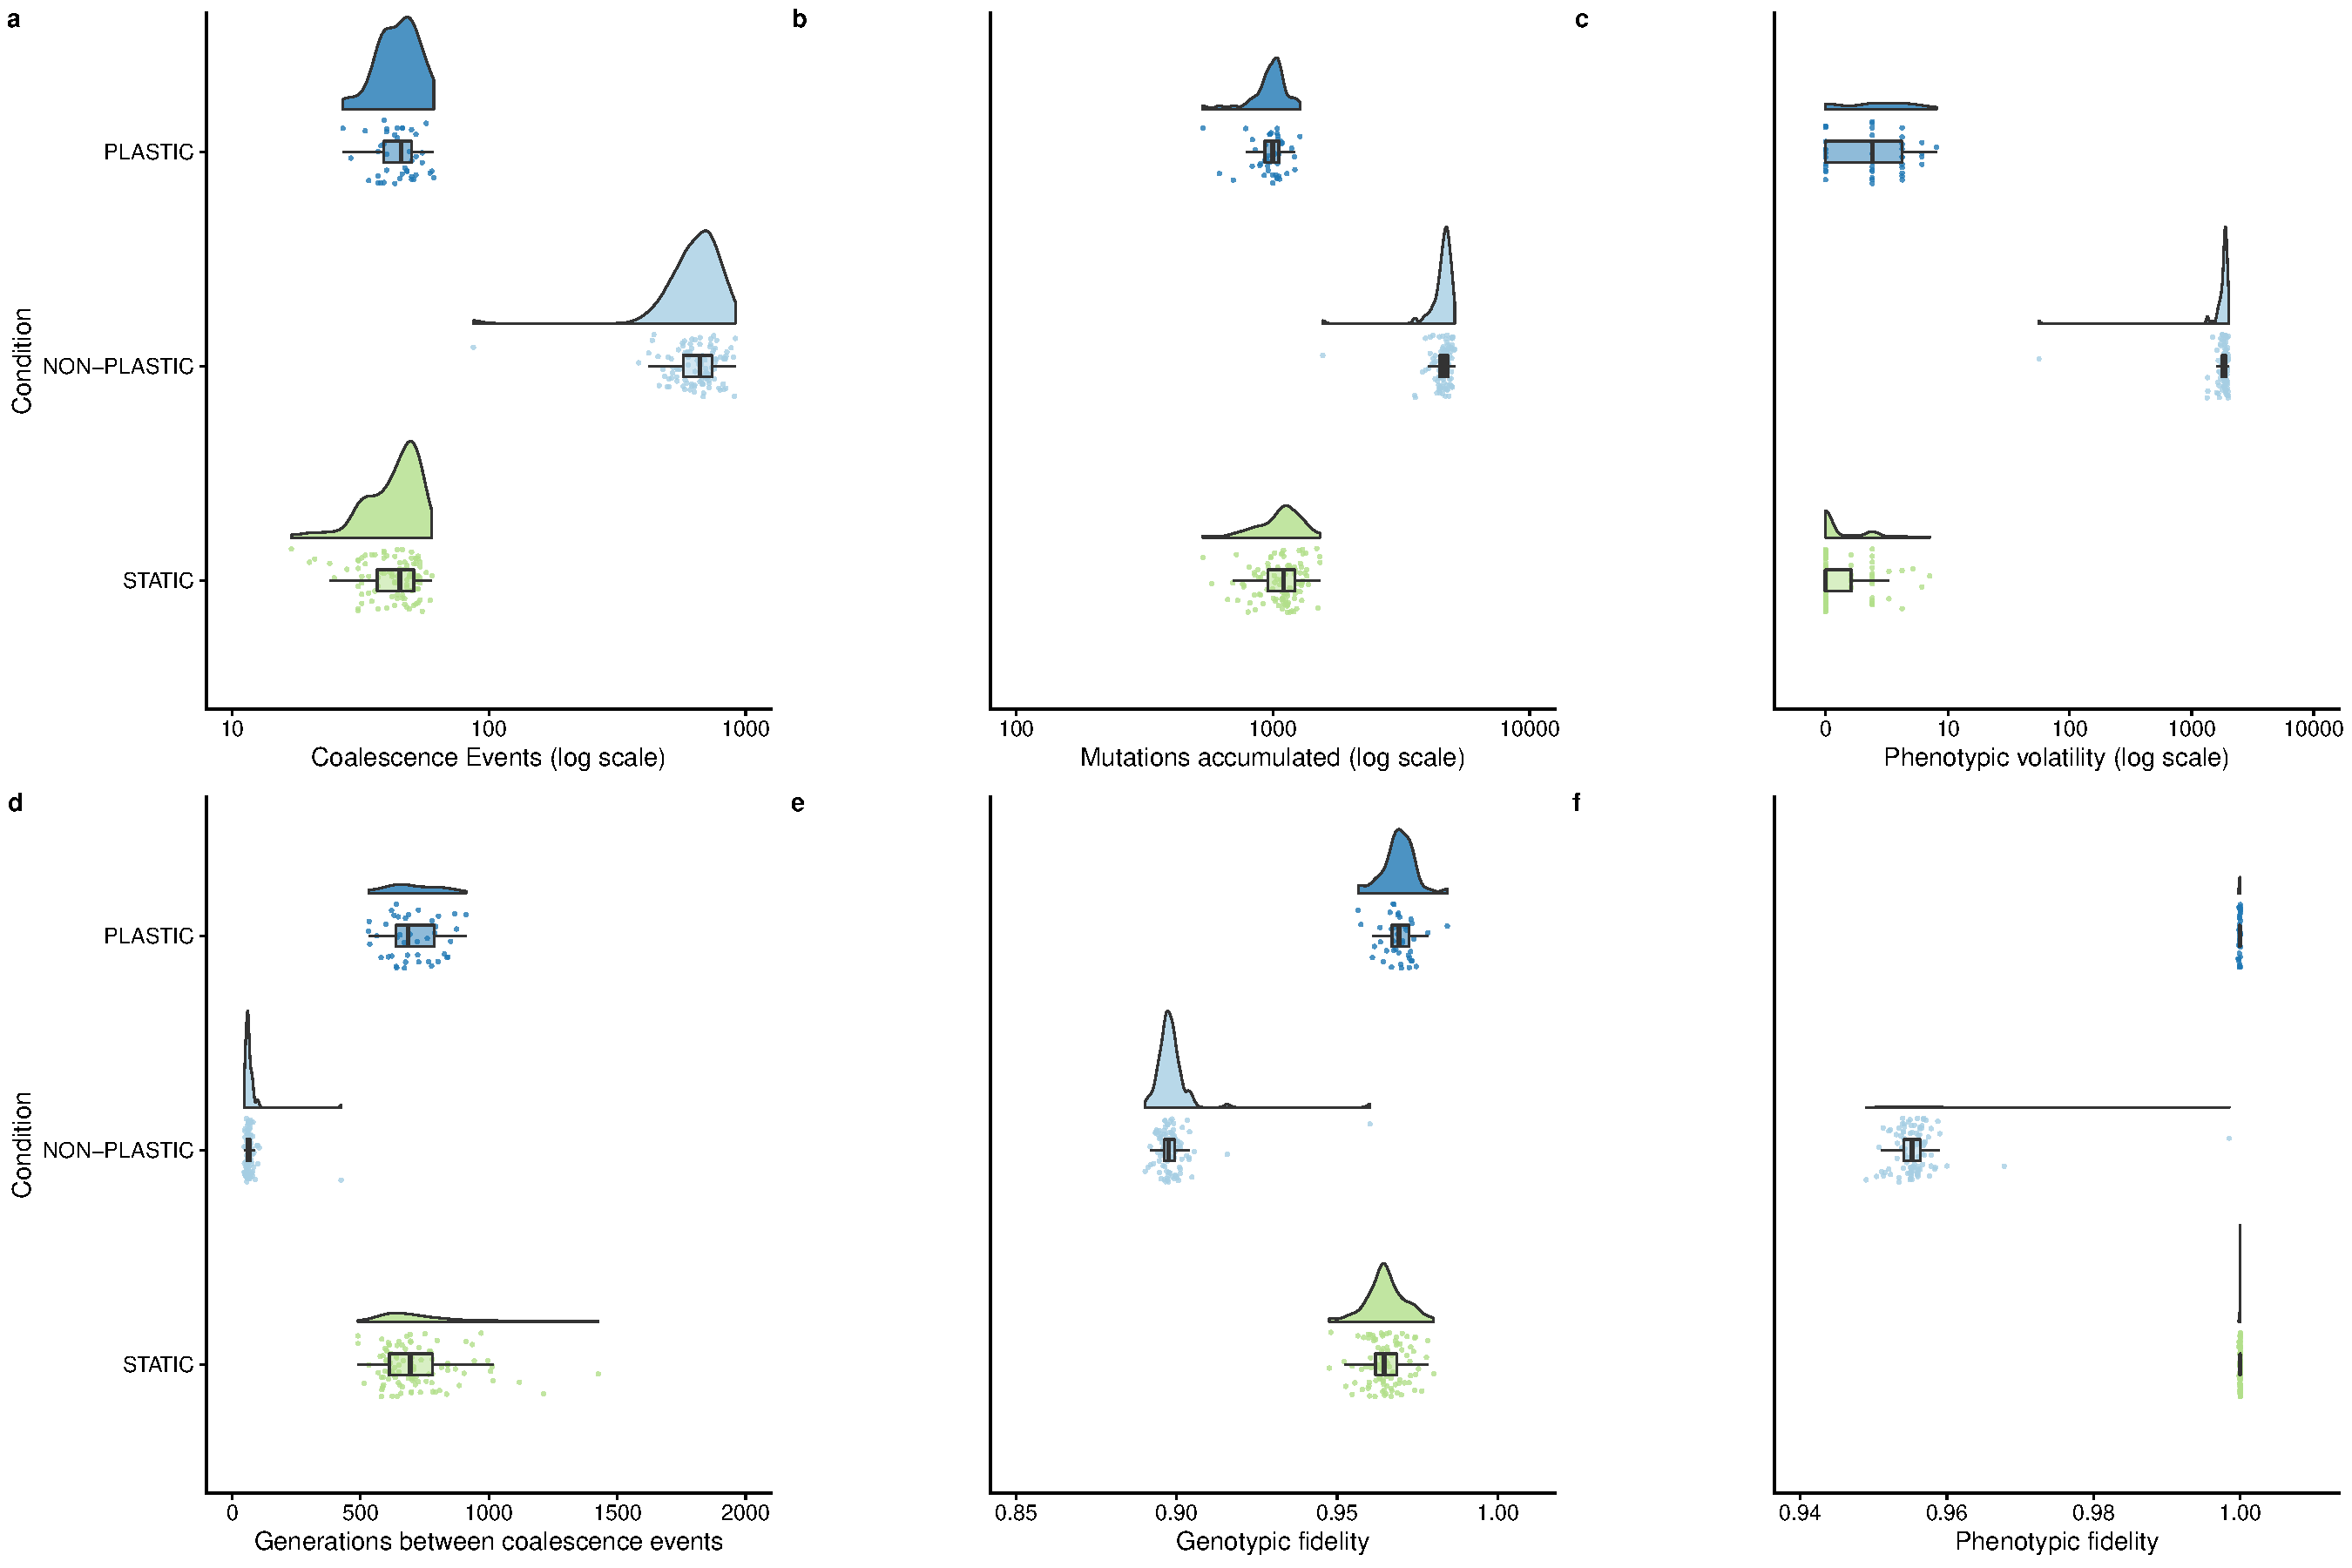
\includegraphics[width=1\textwidth]{media/evolutionary-change-full-panel.pdf}
    \caption{\small
    \textbf{todo title.}
    [Adaptive phenotypic plasticity evolved in \evolutionaryChangeRatePlasticReps\ of \evolutionaryChangeRateReplicates\ replicates from the PLASTIC treatment during phase one of this experiment; we used this more limited group to found the \evolutionaryChangeRatePlasticReps\ phase-two PLASTIC replicates from which we report these PLASTIC data.]
    }
    \label{fig:evolutionary-dynamics}
\end{figure}

\begin{figure}[h!]
    \centering
    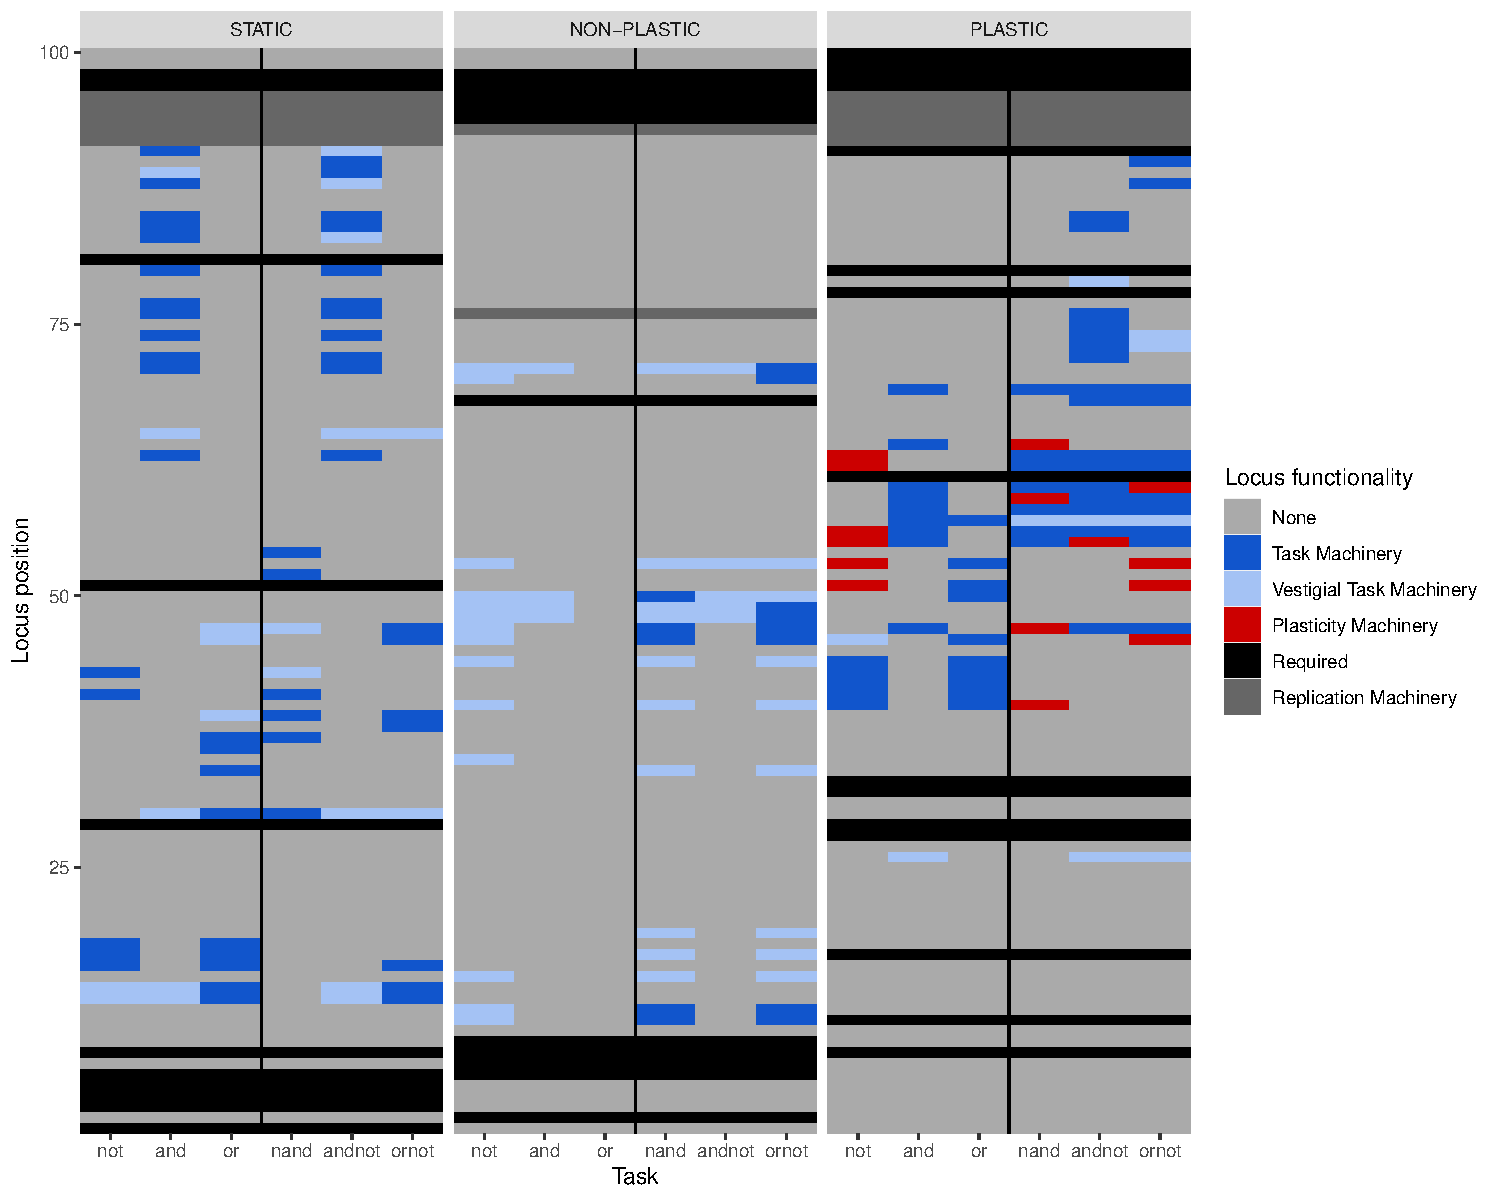
\includegraphics[width=1\textwidth]{media/architecture/locus_slice_combined.pdf}
    \caption{\small
    % TODO: Change "Previous Task Machinery" -> "Vestigial Task Machinery"
    \textbf{todo title.}
    Representative samples from each condition at the end of phase two. 
    The 100-loci genome of each sample is shown, with colors indicating what functionality a locus has for each of the six base tasks. 
    % ENV-A is on the left of the black line (for future reference in writing this)
    % STATIC replicates typic
    }
    \label{fig:architecture_locus_functionality}
\end{figure}
\begin{figure}[ht!]
    \centering
    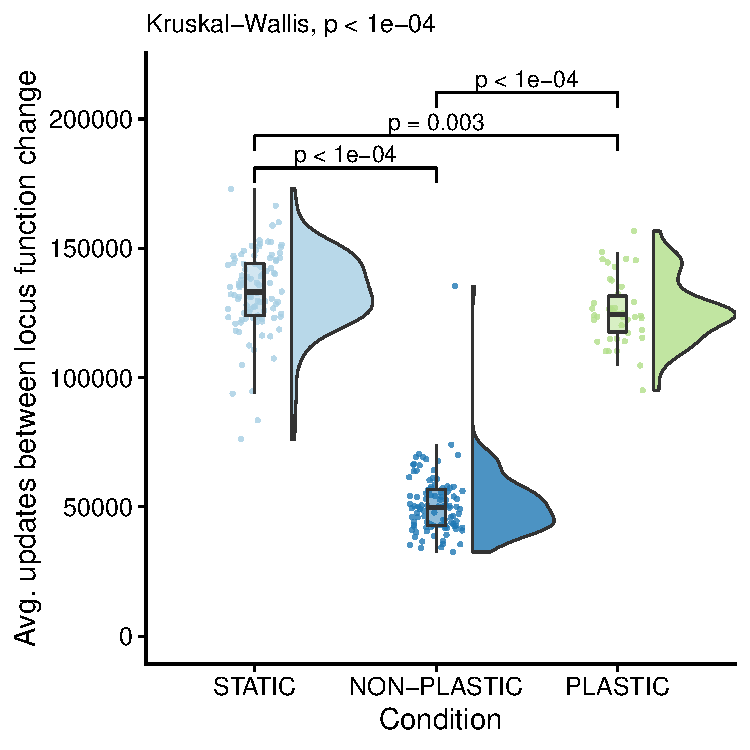
\includegraphics[width=0.33\textwidth]{media/architecture/avg_time_between_func_changes_weighted_mean.pdf}
    \caption{\small
        \textbf{todo title.}
        [todo]
    }
    \label{fig:architecture_locus_change_time}
\end{figure}

%%%%%%%%%%%%%%%%%%%%%%%%%%%%%%%%%
% Results to report (2021-02-08 experiment)
% ----- GENERATIONS -----
% - average generations elapsed (of a population)
%   - NON-PLASTIC (median: 41768.65) > PLASTIC (median: 31697.65) > STATIC (median: 30839.75)
%   condition     mean    sd
%   <chr>        <dbl> <dbl>
% 1 NON-PLASTIC 41090. 2702.
% 2 PLASTIC     31016. 2615.
% 3 STATIC      30002. 3011.

% 
% ----- SWEEPS -----
% - coalescence events (total)
%   - NON-PLASTIC (median: 663.5) > ( PLASTIC (median: 45.5) ~~ STATIC (median: 45) )
% - Average number of generations between coalescence events (gens / sweeps)
%   - ( PLASTIC (median: 685.001780758557) ~~ STATIC (median: 693.676265008576) ) > NON-PLASTIC (median: 62.0184902295191) 
% 
% ----- PHENOTYPIC VOLATILITY -----
% - phenotypic volatility (total)
%   - i.e., total number of times phenotypes change along lineages
%   - NON-PLASTIC (median: 1868) > PLASTIC (median: 2) > STATIC (median: 0)
% - phenotypic volatility / lineage length
%   - i.e., how often do genomic changes reflect changes in phenotype? 
%   - NON-PLASTIC (median: 0.437) > PLASTIC (median: 0.0022) > STATIC (median: 0)
% - phenotypic volatility / generations
%   - i.e., per-offspring rate of phenotypic changes
%   - NON-PLASTIC (median: 0.0447) > PLASTIC (median: 6.33e-05) > STATIC (median: 0)
% 
% ----- MUTATION ACCUMULATION -----
% - mutation accumulation (total)
%   - NON-PLASTIC (median: 4657.5) > STATIC (median: 1100) > PLASTIC (median: 998.5)
% - mutation accumulation / lineage length
%   - NON-PLASTIC (median: 1.10048311715591) > STATIC (median: 1.03794597464116) > PLASTIC (median: 1.0328599144651) 
% - mutation accumulation / generation
%   - NON-PLASTIC (median: 0.11) > STATIC (median: 0.0368) > PLASTIC (median: 0.0319) 
% 
% ----- MUTATIONAL EFFECTS -----
% - fraction of mutational steps that alter (aggregate) phenotype
%   - NON-PLASTIC (mean: 0.434007, CI [0.4242,  0.4406]) > PLASTIC (mean: 0.002717008, 0.0020,  0.0035) > STATIC (mean: 0.0006788834, CI [0.0004,  0.0009])
% - fraction of phenotype-altering mutation steps that alter unexpressed phenotype (PLASTIC condition only)
%   - mean: 0.8247126 CI [0.7443,  0.8994]
% - fraction of mutations that affect unexpressed phenotype that are deleterious (PLASTIC only)
%   - mean: 0.5172414 CI [0.4402,  0.5977]
% - fraction of mutations that affect unexpressed phenotype that are beneficial (PLASTIC only)
%   - mean: 0.4827586 CI [0.4046,  0.5598]
%%%%%%%%%%%%%%%%%%%%%%%%%%%%%%%%%

% -- Magnitude of evolutionary change --
%  - Selective sweeps
%  - Mutation accumulation
%  - Phenotypic volatility
%  - Number of generations elapsed
In experimental \hyperref[sec:methods:exp:evolutionary-change-rate]{phase 2A},
we tested whether the evolution of adaptive phenotypic plasticity constrained or promoted subsequent evolutionary change in a fluctuating environment. 
First, we compared the total amount of evolutionary change in populations evolved under the PLASTIC, NON-PLASTIC, and STATIC treatments as measured by  coalescence event count, mutation count, and phenotypic volatility (Figure \ref{fig:evolutionary-dynamics}).
According to each of these metrics, NON-PLASTIC populations experienced a larger magnitude of evolutionary change than either PLASTIC or STATIC populations.
We observed significantly higher coalescence event counts in NON-PLASTIC populations than in PLASTIC or STATIC populations (Figure \ref{fig:evolutionary-dynamics}\hyperref[fig:evolutionary-dynamics]{a}).
NON-PLASTIC lineages had significantly higher mutation counts (Figure \ref{fig:evolutionary-dynamics}b) and phenotypic volatility than PLASTIC or STATIC lineages (Figure \ref{fig:evolutionary-dynamics}c).

% -- Elapsed generations --
Changing environments have been shown to increase generational turnover in Avida populations \citep{canino-koning_evolution_2016}, which could explain why we observe a larger magnitude of evolutionary change at the end of 200,000 updates of evolution in NON-PLASTIC populations. % because ... large fitness differentials... 
Indeed, we found that significantly more generations of evolution elapsed in NON-PLASTIC populations (mean of $41090\pm2702$ std. dev.) than in PLASTIC (mean of $31016\pm2615$ std. dev.) or STATIC (mean of $30002\pm3011$ std. dev.) populations during phase 2A (corrected Wilcoxon rank-sum tests, p $<10^{-4}$) %, PLASTIC: p $<10^{-4}$; STATIC: p $<10^{-4}$).

% Additionally, we found that significantly more generations of evolution elapsed in NON-PLASTIC populations (mean of $41090\pm2702$ std. dev.) than in PLASTIC (mean of $31016\pm2615$ std. dev.) or STATIC (mean of $30002\pm3011$ std. dev.) populations during phase 2A (corrected Wilcoxon rank-sum tests, PLASTIC: p $<10^{-4}$; STATIC: p $<10^{-4}$).
%; that is, NON-PLASTIC populations exhibited a higher rate of generational turnover (mean of $41090\pm2702$ std. dev.) than PLASTIC (mean of $31016\pm2615$ std. dev.) or STATIC (mean of $30002\pm3011$ std. dev.) populations in the given 200,000 Avida updates.

% -- Rate of evolutionary change => intuition --
%   - Rate of sweeps => (generations per sweep)
%   - genotypic fidelity => frequency that offspring's genotype is identical to parent genotype (lineage length / number generations)
%   - phenotypic fidelity => frequency that an offspring's phenotype is same as parent's phenotype (phenotypic volatility / number of generations)
To evaluate whether increased generational turnover explains the greater magnitude of evolutionary change in NON-PLASTIC populations, we examined the average number of generations between coalescence events and the mutational stability of lineages (Table \ref{tab:metrics-definitions}).
% the \textit{rate} of evolutionary change in PLASTIC, STATIC, and NON-PLASTIC populations. 
% Specifically, we calculated the average number of generations between coalescence events and mutational stability (Table \ref{tab:metrics-definitions}).
% The rate that coalescence events occur can indicate the strength of selection \citep{dolson_interpreting_2020}.
% For example, we would expect populations evolving under strong directional selection to experience more rapid coalescence events than populations evolving under weak selection pressure.
A coalescence event indicates a selective sweep, which is a hallmark of adaptive evolutionary change.
% Genotypic and phenotypic fidelity measure the frequency that an offspring's genotype or phenotype is identical to that of its parent along a given lineage.
Mutational stability measures the frequency that mutations cause phenotypic changes along a lineage.
% We hypothesize that the STATIC treatment produces highly fit genotypes that no longer undergo rapid adaptive change and hence do not trigger frequent coalescence events.
We expect that static conditions should favor fit lineages with high mutational stability that no longer undergo rapid adaptive change and hence do not trigger frequent coalescence events.
Under fluctuating conditions, however, lineages must be composed of plastic organisms if they are to maintain high fitness and mutational stability.
Without plasticity, we expect these conditions to produce lineages with low stability and frequent coalescence events as populations must continually readapt.

% Given , the lineages of organisms evolved in static conditions should exhibit high genotypic and phenotypic fidelity.

% and have high genotypic and phenotypic fidelity.
% than those evolved under changing conditions, as changing conditions require populations to continuously adapt.

% if more selective sweeps occurred, indication of adaptive evolution 
% adaptive evolutionary change

% -- Rate of evolutionary change => findings --
On average, significantly fewer generations elapsed between coalescence events in NON-PLASTIC populations than in either PLASTIC or STATIC populations (Figure \ref{fig:evolutionary-dynamics}d).
We also observed that PLASTIC and STATIC lineages had significantly higher genotypic and phenotypic fidelity than NON-PLASTIC lineages (Figure \ref{fig:evolutionary-dynamics}e and \ref{fig:evolutionary-dynamics}f, respectively); that is, offspring were identical to their parent more often in the PLASTIC and STATIC regimes than in the NON-PLASTIC regime.
Overall, our results indicate that NON-PLASTIC populations underwent more rapid (and thus a greater amount of) evolutionary changes than either PLASTIC or STATIC populations. 

% -- mutations affect phenotypes --
%   - fraction of mutational steps that alter (aggregate) phenotype
%   - fraction of phenotype-altering mutation steps that alter unexpressed phenotype (PLASTIC condition only)
%   - fraction of mutations that affect unexpressed phenotype that are deleterious (PLASTIC only)
%   - fraction of mutations that affect unexpressed phenotype that are beneficial (PLASTIC only)
% @AML: TODO - update with mutational stability
%   - IDEA: Terms for over 30 years working with digital evolution


% the nature of the evolutionary changes observed under the PLASTIC, NON-PLASTIC, and STATIC treatment regimes.
% Specifically, we performed knockout experiments to characterize evolved genetic architectures.
% genetic architectures of representative organisms and how those architectures changed over time.
% Mutational stability combines the information from genotypic and phenotypic fidelity, measuring the proportion of \textit{mutated} offspring whose phenotypic profile matches that of their parent; that is, how often do mutations actually effect phenotypic changes along a given lineage?
% For example, lineages that exhibit frequent mutationally-induced phenotypic changes will have low mutational stability relative to lineages that exhibit little to no mutationally-induced phenotypic changes.

% Consistent with both genotypic and phenotypic fidelity, we found that both STATIC and PLASTIC lineages exhibited high mutational stability relative to that of NON-PLASTIC lineages (corrected Wilcoxon rank-sum tests, PLASTIC: p $<10^{-4}$; STATIC: p $<10^{-4}$).
% [Specifically, non-plastic offspring more often had a different phenotype (mean +- std dev)].
% We also found that STATIC lineages exhibited higher mutational stability than PLASTIC lineages (corrected Wilcoxon rank-sum test, p $<10^{-4}$), which we hypothesized was due to the possibility for cryptic variation to manifest in the off-environment phenotypes of plastic organisms. 
% We found that STATIC lineages exhibited a small, but significant
% Because our 
% While mutational stability for PLASTIC and STATIC lineages is higher than that of NON-PLASTIC lineages, we found that STATIC lineages exhibit a small, but significant, difference in mutational stability relative to PLASTIC lineages [stats]. 
% Overall, there were few instances of mutations that caused a change in phenotypic profile across all PLASTIC lineages.
% However, of these mutations, we found that over 80\% (83 out of 102) of changes to phenotypic profiles was cryptic; that is, they occurred in traits that would not have been expressed when the organism was alive but would have been expressed if the environment changed.

% -- genetic architectures --
% - Since we're looking at the phenotypic profile, we see that STATIC and PLASTIC treatments perform tasks in both environments while NON-PLASTIC only perform tasks from one environment
    % - Like we'd expect!
% - Additionally, we see substantial vestigial task machinery in the NON-PLASTIC treatment, showing that a small number of mutations can cause the task profile to flip environments
% - Indeed, we see that the NON-PLASTIC treatment sees loci functionality change much more frequently. 

% --- BOOKMARK ---
Next, we performed knockout experiments to investigate how genetic architectures evolved under the PLASTIC, NON-PLASTIC, and STATIC treatment regimes.
Figure \ref{fig:architecture_locus_functionality} shows the functionality of each locus in the most abundant genotype of the final population, using a representative sample from each treatment. 
PLASTIC and STATIC genomes perform tasks in both environments, while the NON-PLASTIC genome only performs tasks in the B environment.
We see substantial vestigial task machinery in environment A for the NON-PLASTIC genome, indicating that the genome previously performed environment A tasks but some other locus changed to ``switch off'' those tasks while leaving the sites intact.  
Indeed, Figure \ref{fig:architecture_locus_change_time} demonstrates that, when looking at locus functionality over an entire lineage, loci change function significantly faster (and thus more often) in the NON-PLASTIC treatment [stats].
%This supports our hypothesis that NON-PLASTIC populations rely on [genetic re-adaptation] to [keep up with] the changing environment, while the PLASTIC and STATIC treatments have relatively fixed architecture. 
This supports our hypothesis that the fluctuating environment forces NON-PLASTIC populations to rely on mutations to continuously readapt, while organisms that are adaptively plastic change their phenotype according to environmental stimuli and thus do not require genetic changes to readapt. 


% -- in general, PLASTIC and STATIC more similar than NON-PLASTIC --
In general, the evolution of adaptive plasticity stabilized PLASTIC treatment populations against environmental fluctuations, and their evolutionary dynamics more closely resembled those of populations evolving in a static environment.
We observed no significant difference in the number and frequency of coalescence events in PLASTIC and STATIC populations.
We did, however, observe small, but statistically significant, differences in each of elapsed generations, mutation counts, genotypic fidelity, phenotypic fidelity, and mutational stability between PLASTIC and STATIC populations (see supplemental material \citealt{supplemental_material}).

\vspace{0.5cm}
\subsection{Adaptively plastic populations retain more novel tasks than non-plastic populations in fluctuating environments}

%%%%%%%%%%%%%%%%%%%%%%%%%%%%%%%%%
% Results to report (2021-01-31)
% - Number of plastic replicates
% - Final dominant genotype # novel traits
%   - non-plastic < (plastic == static)
% - Final population (1% threshold): 
%   - non-plastic < plastic < static
% - Final population (1% threshold) discovered:
%   - non-plastic > (plastic ~~ static)
% - Lineage tasks discovered
%   - non-plastic > static ~>(nosig) plastic
% - Lineage tasks discovered / step
%   - (static ~~ plastic) > non-plastic 
% - Lineage tasks lost
%   - non-plastic > static > plastic
% - Lineage tasks lost / step
%   - non-plastic > static > plastic

% - tasks discovered per generation(?)
%   - NON-PLASTIC [0.00014358046266055] ~~ STATIC [0.00015363220504867] > PLASTIC [0.000117695011124939]
% - tasks lost per generation(?)
%   - NON-PLASTIC [0.0022026054610079] > STATIC [0.000161396283669756] > PLASTIC [6.25141973661864e-05]
%%%%%%%%%%%%%%%%%%%%%%%%%%%%%%%%%

\begin{figure}[h!]
    \centering
    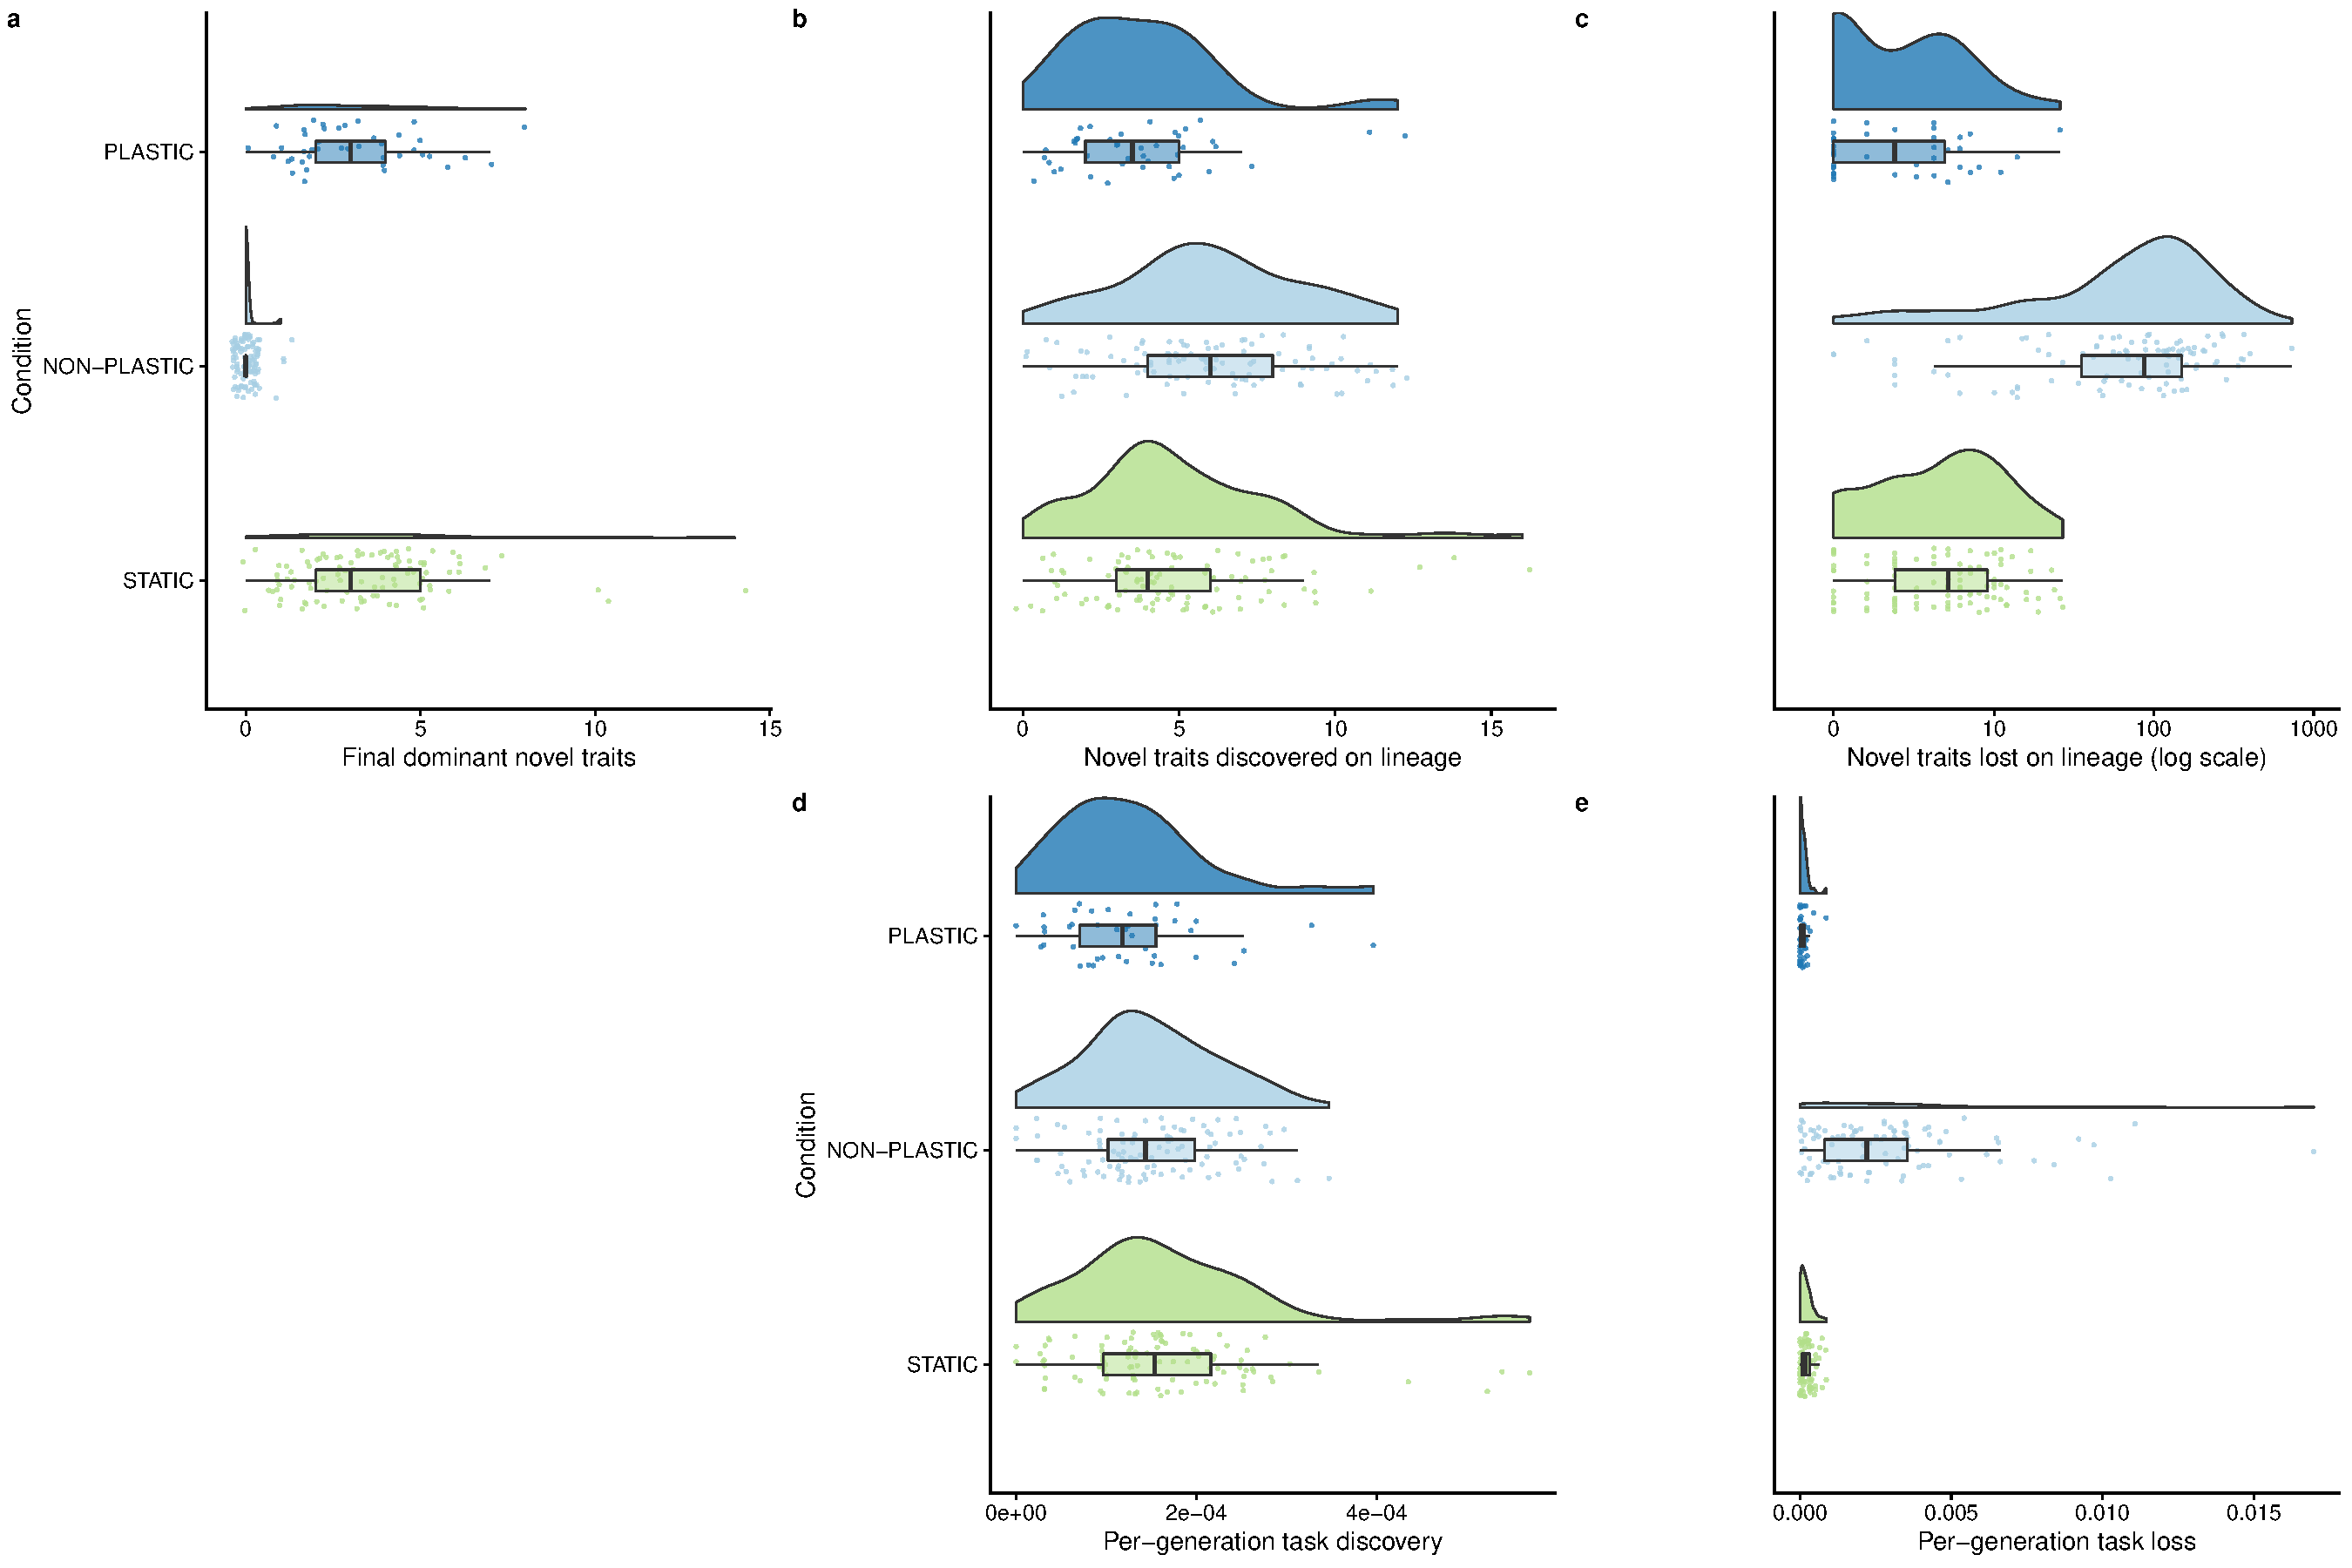
\includegraphics[width=0.9\textwidth]{media/complex-traits-panel.pdf}
    \caption{\small
    \textbf{todo title.}
    todo.
    }
    \label{fig:complex-traits}
\end{figure}

% [Environmental change has been shown to drive evolutionary change and promote evolutionary exploration in non-plastic populations as compared to populations evolving in an unchanging environment \citep{zaman_coevolution_2014,nahum_improved_2017}.]
% [If so, does adaptive plasticity negate the [effects of environmental change on evolutionary exploration]? 

% -- What did we test? --
In experimental phase 2B, we evaluated how evolution of adaptive phenotypic plasticity influences the ability of populations to evolve and retain novel adaptive traits.
We have shown that adaptive plasticity constrains the rate of evolutionary change in fluctuating environments.
However, it is unclear how this dynamic influences the evolution of novel tasks.
Based on their relative rates of evolutionary change, we might expect NON-PLASTIC-treatment populations to evolve more novel tasks than PLASTIC-treatment populations.
But, how much of the evolutionary change in NON-PLASTIC-treatment populations is useful for exploring novel regions of the fitness landscape versus repeatedly re-treading previously explored regions of the fitness landscape?

% - Magnitude of exploration/exploitation -
%   - task performance
%   - task discovery
%   - task loss
% Adaptive phenotypic plasticity evolved in \novelTraitsPlasticReps\ of \novelTraitsReplicates\ replicates from the PLASTIC treatment during phase one of Experiment II; we used this more limited group to seed the \novelTraitsPlasticReps\ phase-two PLASTIC replicates.
Figure \ref{fig:complex-traits} shows the final novel task count, novel task discovery, and novel task loss for the PLASTIC, NON-PLASTIC, and STATIC treatments.
Final novel task count measures the number of novel tasks performed by a representative organism in the final population of each replicate, which indicates how well the final population exploits the fitness landscape.
Novel task discovery is the number of types of novel tasks ever performed by an organism along a representative lineage, which sheds light on how well lineages explore the fitness landscape. 
Finally, novel task loss is the number of times along a representative lineage that a novel task is performed by a parent but not its offspring, which measures a lineage's capacity to maintain novel tasks. 

We found that both PLASTIC and STATIC populations had significantly higher final task counts than NON-PLASTIC populations at the end of the experiment (Figure~\ref{fig:complex-traits}a).
This, however, was not due to PLASTIC and STATIC lineages exploring a larger breadth of the fitness landscape, as NON-PLASTIC lineages exhibited significantly higher novel task discovery than either PLASTIC or STATIC lineages (Figure~\ref{fig:complex-traits}b).
Indeed, we found that NON-PLASTIC lineages repeatedly failed to retain evolved novel tasks, exhibiting significantly higher novel task loss than either PLASTIC or STATIC lineages (Figure~\ref{fig:complex-traits}c).

% - Rates of exploration/exploitation -
%  - tasks discovered per generation(?)
%  - tasks lost per generation(?)
As noted previously, a larger number of generations elapsed in NON-PLASTIC populations than in PLASTIC or STATIC populations during our experiment.
Are NON-PLASTIC lineages discovering and losing novel tasks more frequently than PLASTIC or STATIC lineages, or are our observations a result of differences in generational turnover?
To tease this apart, we examined the frequencies of novel task discovery and novel task loss along representative lineages by dividing novel task discovery and novel task loss measurements by the number of elapsed generations.
We found no significant difference in the frequency of novel task discovery between NON-PLASTIC and STATIC lineages, and we found that PLASTIC lineages had a lower frequency of novel task discovery than STATIC lineages (Figure~\ref{fig:complex-traits}d).
Therefore, we cannot reject the possibility that the larger magnitude of task discovery in NON-PLASTIC lineages was driven by a larger number of elapsed generations.
NON-PLASTIC lineages had a higher frequency of task loss than either PLASTIC or STATIC lineages, and PLASTIC lineages tended to have a lower frequency of novel task loss than STATIC lineages (Figure~\ref{fig:complex-traits}e). 

% We computed the per-generation rate of task discovery along dominant lineages and the per-generation rate of task loss along those same lineages.
% small, but significant, per-generation task discovery rate than NON-PLASTIC or STATIC lineages [stats].
% We found that NON-PLASTIC lineages had a significantly higher per-generation rate of task loss than either PLASTIC or STATIC lineages [stats], while PLASTIC lineages had a small but significantly lower per-generation rate of task loss than STATIC lineages [stats].
% Indeed, we found that NON-PLASTIC lineages repeatedly gained and failed to retain novel tasks during the experiment, and the final evolved genotypes performed fewer overall tasks.

% - Characterizing trait loss -
%   - fraction of novel trait loss co-occuring with change in base trait profile
%   - reporting overall aggregate vs. comparing distributions of fractions (among lineages that have trait loss)
% @AML: [Some rationale for doing this???]
Next, we examined the frequency at which novel task loss along lineages co-occurred with a change in base task performance (\textit{i.e.}, the loss or gain of any of the six base tasks).
Across all NON-PLASTIC dominant lineages, over 97\% (10998 out of 11229) of instances of novel task loss co-occurred with a simultaneous change in base task profile.
In contrast, across all PLASTIC and STATIC dominant lineages, we observed that approximately 20\% (29 out of 142) and 2\% (13 out of 631), respectively, of instances of novel task loss co-occurred with a simultaneous change in base task profile. 

% In supplemental experiments, we did find that the relative value of fluctuating and novel tasks affected novel task discovery and retention [cite supplement]. 
% While the overall patterns that we observed were consistent, 
% [Limitation (relative value): in supplemental experiments, relative value of fluctuating and novel tasks affects novel task retention, the stronger directional selection on fluctuation tasks relative to selection on novel tasks makes novel tasks harder to maintain because less deleterious to lose novel trait].

\vspace{0.5cm}
\subsection{Non-plastic lineages accumulate more deleterious instructions in fluctuating environments}

%%%%%%
% 2021-02-05 - Results
% - Number of offspring on lineage where hitchhiker instruction execution increases (i.e., instances of hitchhiking)
%   - PLASTIC ~~ STATIC < NON-PLASTIC
% - Hitchhiker instruction increases / offspring on lineage
%   - PLASTIC ~~ STATIC < NON-PLASTIC
% - What fraction of mutations that increase hitchhiker instruction execution co-occur with base trait changes?
%   - NON-PLASTIC > PLASTIC ~~ STATIC
% - What about unexpressed vs expressed trait changes in plastic populations? (plastic only)
%   - Not much hitchhiking. Did not find evidence that hitchiking occurring as cryptic variation in unexpressed phenotype.
%%%%%%

% -- what we tested --
% [todo]
% We have shown that adaptive plasticity stabilized populations against environmental fluctuations, which reduced novel trait loss along the lineages of adaptively plastic organisms relative to that of non-plastic organisms. 




% @AML: needs trimming
% the lineages of adaptively plastic organisms accumulate more deleterious \code{poison} instructions than that of non-plastic lineages.
Phenotypic plasticity allows for possibility of accumulating of genetic variation in genomic regions that are unexpressed under contemporary environmental conditions, which could lead to the fixation of deleterious instructions in PLASTIC-treatment populations.
However, our results thus far indicate that PLASTIC-treatment populations accumulate \textit{fewer} deleterious mutations than NON-PLASTIC treatment populations in fluctuating environments.
That is, NON-PLASTIC lineages accumulated more total genetic changes (Figure \ref{fig:evolutionary-dynamics}), and the high rates of novel task loss in NON-PLASTIC lineages (Figure \ref{fig:complex-traits}) may also indicate their increased susceptibility to accumulating deleterious mutations relative to PLASTIC lineages.

In experimental phase 2C, we tested whether the evolution of adaptive phenotypic plasticity increases deleterious instruction accumulation in genomes by measuring poisonous task performance in representative organisms and along representative lineages. 
Organisms can perform the poisonous task by executing a \code{poison} instruction, which reduces their fitness. 
At the beginning of phase two, the \code{poison} instruction is not present in the population as it was not part of the instruction set during the first phase of evolution.
If a \code{poison} instruction fixes in a population, it must be the result of evolutionary dynamics during phase 2C, as no founding organism's genome contained the \code{poison} instruction.
Selection should purge mutations that increase \code{poison} instruction execution in the offspring phenotype, unless those mutations accumulate as cryptic variation in plastic genomes or hitchhike to fixation with linked beneficial mutations.

\begin{figure}[ht!]
    \centering
    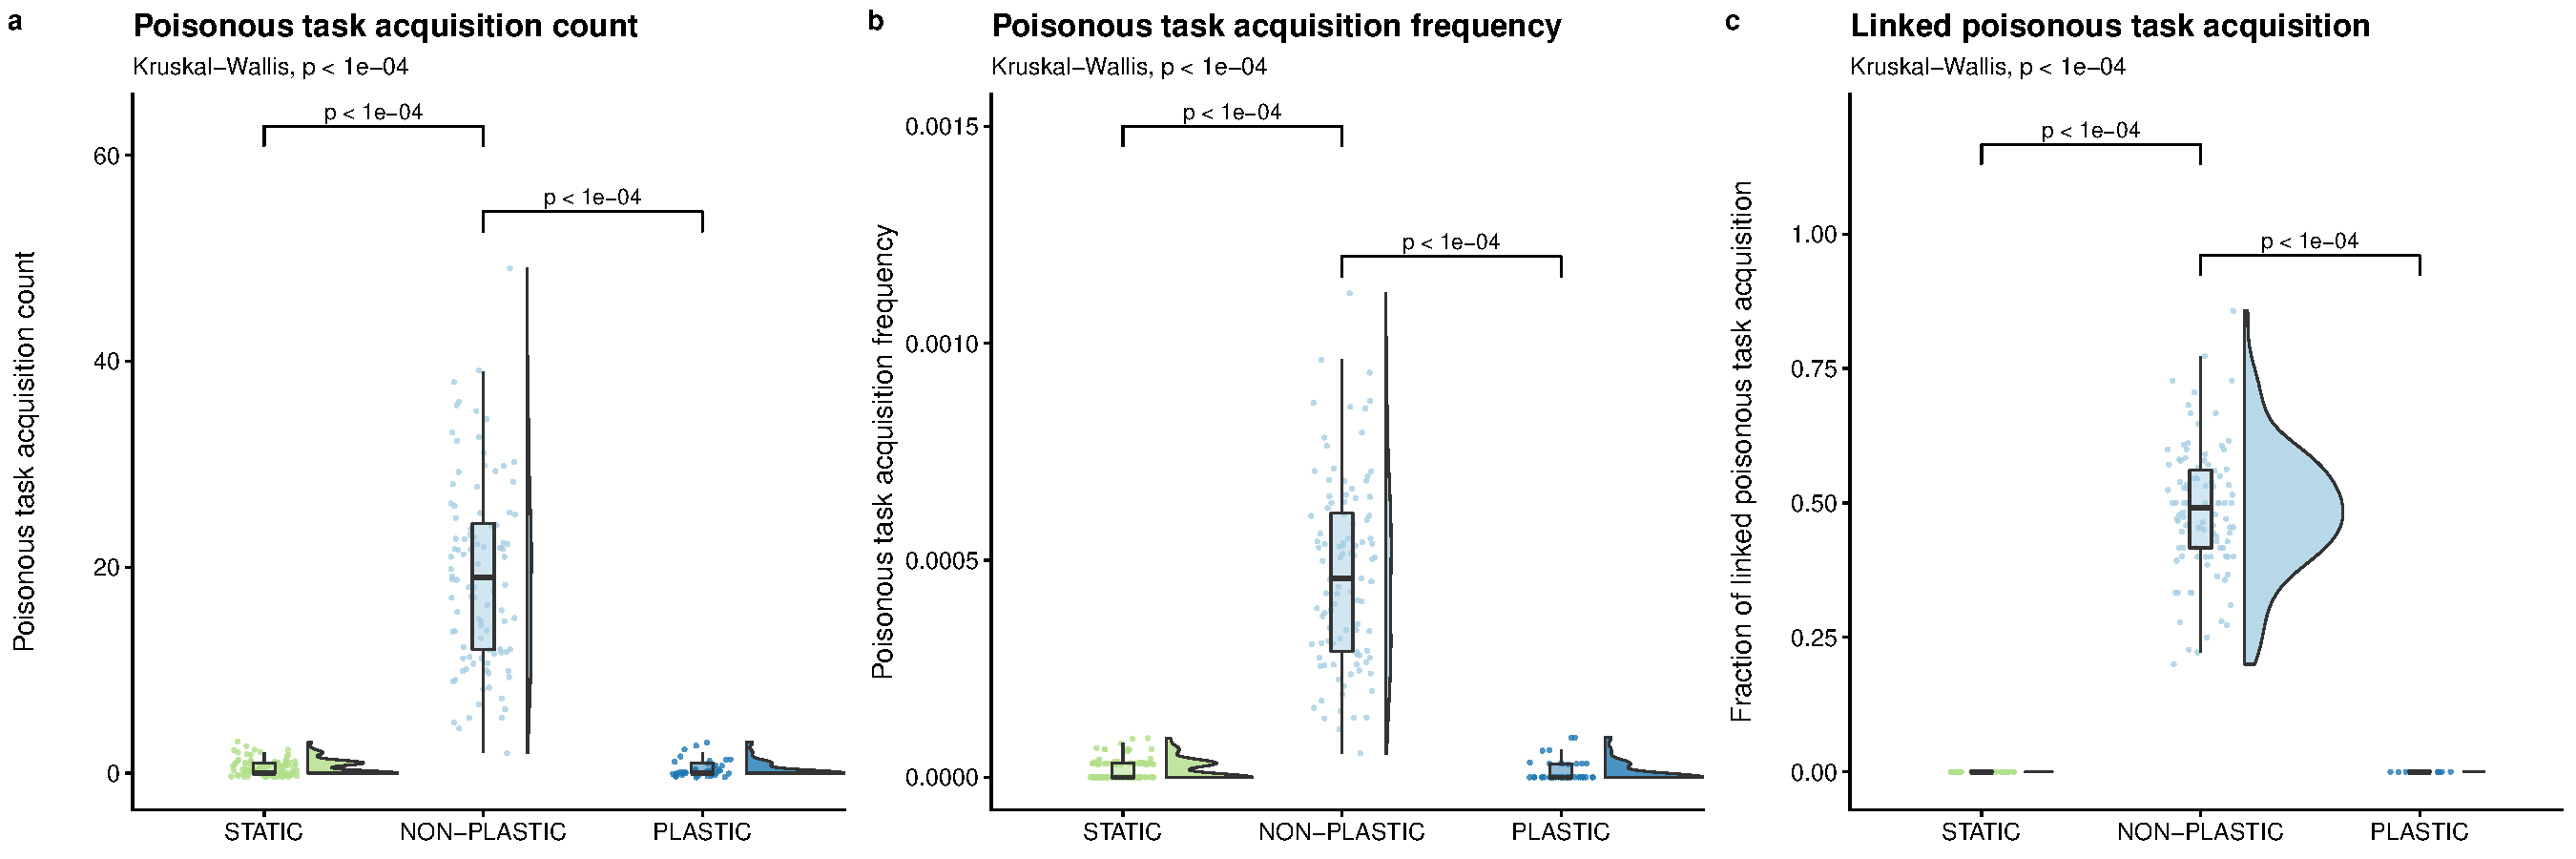
\includegraphics[width=1.0\textwidth]{media/poison-accumulation-panel.pdf}
    \caption{\small
    \textbf{Deleterious instruction accumulation.}
    Raincloud plots of 
    (a) poisonous task acquisition,
    (b) poisonous task acquisition frequency,
    and (c) the proportion of mutations that increase poisonous task performance along a lineage that co-occur with another change in phenotypic profile.
    Each plot is annotated with statistically significant comparisons (Bonferroni-corrected pairwise Wilcoxon rank-sum tests).
    Note that adaptive phenotypic plasticity evolved in \deleteriousHitchhikingPlasticReps\ of \deleteriousHitchhikingReplicates\ replicates from the PLASTIC treatment during phase one of Experiment III; we used this more limited group to seed the \deleteriousHitchhikingPlasticReps\ phase-two PLASTIC replicates.
    }
    \label{fig:deleterious-hitchhiking}
\end{figure}

% -- Instruction execution by final dominant & along lineage --
At the end of our experiment, no representative organisms from the PLASTIC or STATIC treatments performed the poisonous task under any environmental condition; however, representative organisms from 14 replicates of the NON-PLASTIC treatment performed the poisonous task at least once. % (statistically significant, fisher's exact test)
Figure \ref{fig:deleterious-hitchhiking} shows the poisonous task acquisition rate for each treatment, which measures the number of instances along a lineage where a mutation causes an offspring to perform the poisonous task more often than its parent. 
We found that NON-PLASTIC lineages contained significantly more offspring that performed the poisonous task more often than their parent as compared to offspring along PLASTIC or STATIC lineages (\ref{fig:deleterious-hitchhiking}a).
This result does not change when we normalize each poisonous task acquisition value by the number of generations represented in the given lineage (Figure \ref{fig:deleterious-hitchhiking}b).

% -- When/where does hitchhiking take place? --
% @AML: Could use a little transition here!
Next, we examined the frequency that mutations that increase \code{poison} execution co-occurred with mutations that change the base task profile of offspring along representative lineages.
Across all NON-PLASTIC representative lineages, we found that approximately 49\% (956 out of 1916) mutations that increased \code{poison} instruction execution co-occurred with mutations that changed the base task profile.
Along all representative lineages from the PLASTIC treatment, only 18 offspring sustained a mutation that increased task poisonous task performance relative to their parent, and none of these mutations simultaneously co-occurred with a change in base task profile.
Likewise, along all representative lineages from the STATIC treatment, only 58 offspring sustained a mutation that increased poisonous task performance, and none of these mutations simultaneously co-occurred with a change in base task profile.
We did not find compelling evidence that the few mutations that increased \code{poison} task performance occurred as cryptic variation in PLASTIC lineages.

We repeated this experiment with 3\% and 30\% metabolic rate penalties associated with the poisonous task, which produced consistent experimental results \citep{supplemental_material}.